\section{Causal Optical Mechanisms and Pre-Deployment Risk Gating (\textbf{RQ2} \& \textbf{RQ3})}
\label{sec:mechanisms}

Having established that shader-induced turnover persists across model scales and four distinct architectures well above path-tracing noise, we next investigate its optical causes (\textbf{RQ2}) and ask whether regressions can be anticipated automatically before invoking any VLM (\textbf{RQ3}).

\subsection{2,880 Cross-Family Silhouette Counterfactuals and Photometric Controls}
\label{sec:counterfactuals}

Explaining material sensitivity from natural conversion pairs alone faces two confounds: foreground--background edits over rectangular boxes mix surrounding context inside the box, and simple shifts in object brightness or color can change visual salience \citep{Burgert2025NotTexture} independently of higher-order shader properties. To isolate these optical channels without introducing fresh path-tracing noise, we construct \textbf{three pixel-exact counterfactuals} for every pair (1,440 images) from the frozen renders and simulator segmentation masks $M_i^v$, evaluating all conditions on \emph{two independent 8B architectures} (\textsc{Qwen3-VL-8B} and \textsc{InternVL3.5-8B-HF}; \textbf{2,880 evaluations total}):
\begin{enumerate}
    \item \textbf{Target-only shader conversion ($I_i^T$):} Pixels inside the converted target mask $M_i^C$ take \converted\ values while the background remains \original, using symmetric boundary compositing where mask edges differ in 7/480 pairs.
    \item \textbf{Background-only shader conversion ($I_i^B$):} Pixels inside $M_i^O$ remain \original\ while surrounding scene context takes \converted\ values.
    \item \textbf{Photometric-matched control ($I_i^{\text{photo}}$):} Starting from $I_i^O$, affine channel matching in $\mathrm{CIE}~L^*a^*b^*$ aligns target and background color and luminance means and standard deviations separately to $I_i^C$, while preserving native \textsc{MDL} textures, specular reflections, and high-frequency detail.
\end{enumerate}

\begin{table*}[!t]
\centering\scriptsize
\resizebox{\textwidth}{!}{% Verified from paper/shared/evidence/raw/cviu_v3/optical_mechanisms.json (2,880 counterfactual evaluations)
\begin{tabular}{@{}lrrrrrrrrrrr@{}}
\toprule
Condition / Optical Stratum & $N$ & \multicolumn{5}{c}{Qwen3-VL-8B (1,440 CF evals)} & \multicolumn{5}{c}{InternVL3.5-8B-HF (1,440 CF evals)} \\
\cmidrule(lr){3-7} \cmidrule(lr){8-12}
 & & $H$ (\%) & Flip [95\% CI] & L / G (\%) & Shift & Net $\Delta$ & $H$ (\%) & Flip [95\% CI] & L / G (\%) & Shift & Net $\Delta$ \\
\midrule
\multicolumn{12}{@{}l}{\emph{Panel A: 480-pair natural counterfactual decomposition (2,880 synthesized CF evaluations across 2 independent 8B families)}} \\
Original (\textsc{MDL}) $I^O$ & 480 & 81.25 & --- & --- & --- & --- & 78.54 & --- & --- & --- & --- \\
Photometric ($\mathrm{CIE}~L^*a^*b^*$) $I^{\text{photo}}$ & 480 & 80.83 & 5.83 [3.75, 8.13] & 3.13 / 2.71 & 20.27 & -0.42 & 79.38 & 7.08 [5.00, 9.38] & 3.13 / 3.96 & 32.26 & +0.83 \\
Background-converted only $I^B$ & 480 & 80.63 & 6.46 [4.58, 8.54] & 3.54 / 2.92 & 23.37 & -0.63 & 80.21 & 9.17 [6.67, 11.88] & 3.75 / 5.42 & 38.97 & +1.67 \\
Target-converted only $I^T$ & 480 & 80.63 & 8.13 [5.63, 10.83] & 4.38 / 3.75 & 24.16 & -0.63 & 81.25 & 9.79 [7.29, 12.50] & 3.54 / 6.25 & 37.47 & +2.71 \\
Full converted (\texttt{Preview}) $I^F$ & 480 & 83.13 & \textbf{9.38} [7.08, 11.67] & 3.75 / 5.63 & 27.23 & +1.88 & 80.00 & \textbf{10.63} [7.92, 13.54] & 4.58 / 6.04 & 47.11 & +1.46 \\
\midrule
Non-photometric residual ($I^F - I^{\text{photo}}$, 480) & 480 & +2.29 & \textbf{+3.54} [+1.25, +5.83] & +0.63 / +2.92 & +6.96 & --- & +0.63 & \textbf{+3.54} [+1.04, +6.04] & +1.46 / +2.08 & +14.85 & --- \\
Non-photometric residual (473 id.-mask) & 473 & +2.11 & \textbf{+3.38} [+1.26, +5.70] & +0.63 / +2.75 & +6.98 & --- & +0.42 & \textbf{+3.38} [+0.84, +5.97] & +1.48 / +1.90 & +14.79 & --- \\
\midrule
\multicolumn{12}{@{}l}{\emph{Panel B: Paired stratification of Full ($I^F$) vs.\ Original ($I^O$) by prior surface optical regime}} \\
Reflective / Metallic & 158 & 79.75 & 10.76 & 3.16 / 7.59 & --- & \textbf{+4.43} & 77.85 & 10.76 & 5.06 / 5.70 & --- & +0.63 \\
Transparent / Glass & 176 & 84.66 & 9.66 & 4.55 / 5.11 & --- & +0.57 & 85.80 & 9.66 & 3.98 / 5.68 & --- & +1.70 \\
Matte / Diffuse & 88 & 86.36 & 10.23 & 4.55 / 5.68 & --- & +1.14 & 75.00 & 10.23 & 5.68 / 4.55 & --- & \textbf{-1.14} \\
Emissive / Screen & 58 & 82.76 & 3.45 & 1.72 / 1.72 & --- & +0.00 & 75.86 & 13.79 & 3.45 / 10.34 & --- & \textbf{+6.90} \\
\bottomrule
\end{tabular}
}
\caption{Cross-family causal optical decomposition on \textsc{Qwen3-VL-8B} and \textsc{InternVL3.5-8B-HF} over all 480 natural pairs (2,880 total counterfactual inferences), sensitivity check on 473 bit-identical mask pairs, and stratification by prior surface optical category.}
\label{tab:mechanisms_v3}
\end{table*}

\begin{figure*}[!t]
\centering
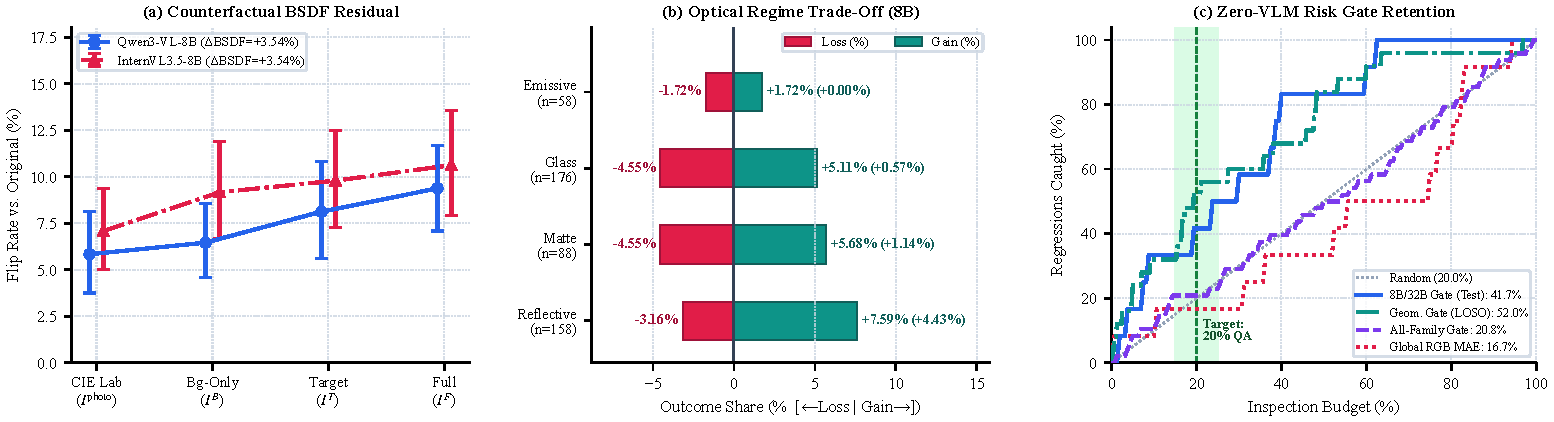
\includegraphics[width=\textwidth]{fig5_causal_and_risk.pdf}
\caption{\textbf{Cross-family optical mechanism decomposition and zero-\textsc{VLM} pre-deployment risk gating (\textbf{RQ2} \& \textbf{RQ3}).}
\emph{(a)} Across 2,880 counterfactual evaluations on \textsc{Qwen3-VL-8B} and \textsc{InternVL3.5-8B-HF}, matched $\mathrm{CIE}~L^*a^*b^*$ luminance/color salience ($I^{\text{photo}}$) leaves an identical \textbf{$+3.54\%$} non-photometric \textsc{BSDF} flip residual ($I^F - I^{\text{photo}}$) on both independent families.
\emph{(b)} Surface optical regimes explain mean-delta cancellation on \textsc{Qwen3-VL-8B}: \emph{Reflective/Metallic} targets gain $+4.43\%$ via glare suppression ($7.59\%$ Gain vs.\ $3.16\%$ Loss), whereas \emph{Transparent/Glass} and \emph{Matte/Diffuse} trade regressions against improvements.
\emph{(c)} Zero-\textsc{VLM} selective quality-assurance curves: routing the highest-risk $20\%$ of pairs captures $41.7\%$ of held-out \textsc{Qwen3-VL} regressions ($52.0\%$ in 30-scene \textsc{LOSO}) vs.\ $16.7\%$ for global \textsc{RGB MAE}, whereas pooling heterogeneous architectures (\texttt{Any-Family}) lowers \textsc{AUROC} ($0.582$ test) because $85.7\%$ of regressions are model-specific.}
\label{fig:mechanisms}
\label{fig:risk_gate}
\end{figure*}

Table~\ref{tab:mechanisms_v3} and Figure~\ref{fig:mechanisms}(a)--(b) yield three consistent optical findings across families:
\begin{itemize}
    \item \textbf{Both 8B architectures exhibit an identical $+3.54\%$ non-photometric BSDF residual.} On \textsc{Qwen3-VL-8B}, matching per-region $\mathrm{CIE}~L^*a^*b^*$ luminance and chromatic moments alone ($I^{\text{photo}}$) accounts for $5.83\%$ flips ($20.27\,\mathrm{px}$ shift; $80.83\%$ hit rate), compared with $9.38\%$ under full shader conversion ($I^F$, $27.23\,\mathrm{px}$), leaving a significant non-photometric residual of \textbf{$+3.54\%$ (95\% CI $[+1.25\%, +5.83\%]$)}. \textsc{InternVL3.5-8B-HF} displays the exact same residual: $I^{\text{photo}}$ induces $7.08\%$ flips ($32.26\,\mathrm{px}$) versus $10.63\%$ under $I^F$ ($47.11\,\mathrm{px}$), again leaving \textbf{$+3.54\%$ (95\% CI $[+1.04\%, +6.04\%]$)}. Restricting to the $473/480$ pairs with bit-identical simulator masks ($\mathrm{IoU}=1.0$) produces virtually unchanged residuals of $+3.38\%$ on both models ($[+1.26\%, +5.70\%]$ on \textsc{Qwen3-VL-8B}; $[+0.84\%, +5.97\%]$ on \textsc{InternVL3.5-8B-HF}).
    \item \textbf{Target dominance and backbone-dependent context coupling.} Both families flip more frequently under target-only shader conversion ($I^T$: $8.13\%$ on \textsc{Qwen3-VL-8B}, $9.79\%$ on \textsc{InternVL3.5-8B-HF}) than background-only conversion ($I^B$: $6.46\%$ and $9.17\%$; paired $T{-}B$ $+1.67\%$ CI $[-0.42\%, +3.96\%]$ and $+0.63\%$ CI $[-1.88\%, +2.92\%]$). Their $2\times 2$ interaction ($I^F - I^T - I^B + I^O$) diverges across models: on \textsc{Qwen3-VL-8B}, isolated target or context swaps modestly reduce accuracy ($81.25\% \to 80.63\%$) before full scene conversion restores illumination coherence ($83.13\%$, interaction $+3.13\%$, CI $[0.00\%, +6.25\%]$), whereas \textsc{InternVL3.5-8B-HF} gains under partial swaps ($80.21\%\text{--}81.25\%$) and settles at $80.00\%$ (interaction $-2.92\%$, CI $[-6.46\%, +0.42\%]$).
    \item \textbf{Optical regime trade-offs behind near-zero aggregate shifts.} Stratifying all 480 pairs by prior surface class (Table~\ref{tab:mechanisms_v3}, Panel~B; Figure~\ref{fig:mechanisms}(b)) reveals the opposing mechanisms that cancel in global averages. On \textsc{Qwen3-VL-8B}, \emph{Reflective/Metallic} targets ($n{=}158$, e.g., stainless appliances and chrome fixtures) improve by $+4.43\%$ ($75.32\% \to 79.75\%$, $7.59\%$ Gain vs.\ $3.16\%$ Loss) as distracting glare recedes, whereas \emph{Transparent/Glass} ($n{=}176$, $+0.57\%$) and \emph{Matte/Diffuse} ($n{=}88$, $+1.14\%$) trade losses against gains; pixel-distortion grouping confirms that \emph{Low-Distortion} captures ($n{=}133$) gain $+3.76\%$ ($84.96\% \to 88.72\%$) while heavily \emph{Specular-Stripped} targets ($n{=}14$) decline $-7.14\%$ ($85.71\% \to 78.57\%$). By contrast, \textsc{InternVL3.5-8B-HF} shows its largest gain on \emph{Emissive/Screen} targets ($n{=}58$, $+6.90\%$, $68.97\% \to 75.86\%$) and a net $-1.14\%$ drop on \emph{Matte/Diffuse} surfaces ($76.14\% \to 75.00\%$).
\end{itemize}

\subsection{Zero-\textsc{VLM} Pre-Deployment Conversion Risk Gate (\textbf{RQ3})}
\label{sec:risk_gate}

Because improvements and regressions stem from distinct optical mechanisms, generic image-difference scores such as global \textsc{RGB MAE} cannot reliably identify hazardous shader exports. We examine whether an automated risk auditor requiring zero \textsc{VLM} inference during export can flag conversion regressions in advance, and how architectural divergence alters gating effectiveness.

For each capture pair, we compute 21 automated cues (\texttt{deploy\_auto}; full inventory in~\ref{app:mechanisms_risk}): five simulator mask-geometry attributes ($\log_{10}$ area fraction, bounding-box aspect ratio, normalized distance from frame center, border-touch indicator, and mask $\mathrm{IoU}$), thirteen paired optical, chromatic, and structural deltas (global/target/background \textsc{RGB MAE}, target lightness and chromatic shifts in $\mathrm{CIE}~L^*a^*b^*$, target lightness-std ratio, target/background \textsc{SSIM}, target Sobel edge ratio, target/ring specular-fraction shifts, and inner/outer contour contrast shifts), and three coarse target-category priors (transparent/glass, reflective appliance/metal, emissive/screen). We fit standardized $\ell_2$-regularized logistic regression on the 15 training scenes ($n{=}240$), select regularization $C$ on the 5 validation scenes ($n{=}80$), and evaluate on the 10 held-out test scenes ($n{=}160$) as well as 30-scene Leave-One-Scene-Out (\textsc{LOSO}) cross-validation across all 480 pairs.

\begin{table*}[!t]
\centering\scriptsize
\resizebox{\textwidth}{!}{% Verified from paper/shared/evidence/raw/cviu_v3/risk_auditor.json
\begin{tabular}{@{}llrrrrrr@{}}
\toprule
Target Regressions & Zero-VLM Predictor / Feature Set & \multicolumn{3}{c}{Held-Out Test (10 scenes, $n{=}160$)} & \multicolumn{3}{c}{30-Scene LOSO ($n{=}480$)} \\
\cmidrule(lr){3-5} \cmidrule(lr){6-8}
 & & AUROC & AUPRC & R@20\% & AUROC & AUPRC & R@20\% \\
\midrule
\multirow{6}{*}{Any 8B/32B Loss (\textsc{Qwen3-VL})} & \texttt{deploy\_auto} (21 automated features) & \textbf{0.743} & 0.195 & 0.417 & 0.653 & 0.137 & 0.360 \\
 & \texttt{geometry\_only} (5 mask features) & 0.742 & \textbf{0.216} & 0.417 & \textbf{0.732} & \textbf{0.184} & \textbf{0.520} \\
 & \texttt{pixel\_only} (13 appearance deltas) & 0.606 & 0.130 & 0.333 & 0.502 & 0.102 & 0.320 \\
 & \texttt{all\_with\_review\_priors} (24 features) & 0.713 & 0.171 & 0.417 & 0.644 & 0.127 & 0.320 \\
 & \texttt{baseline\_target\_rgb\_mae} & 0.557 & 0.172 & 0.417 & 0.577 & 0.140 & 0.280 \\
 & \texttt{baseline\_global\_rgb\_mae} & 0.432 & 0.150 & 0.167 & 0.490 & 0.090 & 0.240 \\
\midrule
\multirow{2}{*}{Qwen3-VL-8B Loss} & \texttt{deploy\_auto} / \texttt{geometry\_only} & 0.632 / 0.650 & 0.080 / 0.092 & 0.286 / 0.143 & 0.594 / 0.666 & 0.077 / 0.096 & 0.389 / 0.389 \\
 & \texttt{baseline\_global\_rgb\_mae} & 0.413 & 0.177 & 0.143 & 0.496 & 0.070 & 0.222 \\
\midrule
Any-Family Loss (6 ckpts pooled) & \texttt{deploy\_auto} / \texttt{geometry\_only} & 0.582 / 0.627 & 0.305 / 0.343 & 0.233 / 0.233 & 0.536 / 0.555 & 0.296 / 0.304 & 0.234 / 0.223 \\
Qwen3-VL-8B Flip (undirected) & \texttt{deploy\_auto} / \texttt{geometry\_only} & 0.501 / 0.601 & 0.103 / 0.130 & 0.062 / 0.250 & 0.545 / 0.537 & 0.117 / 0.125 & 0.244 / 0.200 \\
\bottomrule
\end{tabular}
}
\caption{Zero-\textsc{VLM} pre-deployment conversion risk gating on held-out test scenes ($n{=}160$) and 30-scene \textsc{LOSO} ($n{=}480$). Geometry and paired structural features predict family-specific regressions (\textsc{AUROC} $0.743$ test / $0.732$ \textsc{LOSO}) where global \textsc{RGB MAE} ($0.432$) and undirected \emph{Flip} ($0.501$) fail, whereas pooling heterogeneous losses across all six checkpoints dilutes gating accuracy ($0.582$).}
\label{tab:risk_gate}
\end{table*}

Table~\ref{tab:risk_gate} and Figure~\ref{fig:risk_gate}(c) highlight three design lessons for simulation pipelines:
\begin{enumerate}
    \item \textbf{Why pixel \textsc{MAE} fails and what identifies family-specific risk.} Global \textsc{RGB MAE} reaches only \textsc{AUROC} $= 0.432$ on test scenes ($0.490$ \textsc{LOSO}), worse than random ordering because broad illumination shifts on metallic rooms elevate frame-wide pixel error where grounding actually improves. By contrast, predicting union regression risk within the \textsc{Qwen3-VL} family (\texttt{any\_8b\_32b\_loss}) achieves \textsc{AUROC} $= \mathbf{0.743}$ (95\% CI $[0.597, 0.883]$) using \texttt{deploy\_auto} on test scenes, while \texttt{geometry\_only} achieves \textsc{AUROC} $= \mathbf{0.732}$ (CI $[0.628, 0.837]$) under 30-scene \textsc{LOSO}. Standardized regression weights (\ref{app:mechanisms_risk}) concentrate on small targets (\texttt{log\_area\_frac} $-0.059$), peripheral framing (\texttt{center\_dist\_\allowbreak norm} $+0.058$), internal structural distortion (\texttt{target\_\allowbreak ssim} $-0.035$), and non-metallic surfaces (\texttt{cat\_is\_\allowbreak reflective\_\allowbreak appliance\_\allowbreak or\_\allowbreak metal} $-0.035$).
    \item \textbf{Why gating must be directional and family-calibrated.} Predicting undirected \texttt{8b\_flip} drops test \textsc{AUROC} to $0.501$ because gains and losses respond to opposite visual triggers. Likewise, pooling regressions across all six checkpoints (\texttt{any\_family\_loss}) depresses \textsc{AUROC} to $0.582$ (\texttt{deploy\_auto}) and $0.627$ (\texttt{geometry\_only}) on test scenes ($0.536$ / $0.555$ \textsc{LOSO}; $0.233$ recall at $20\%$). Consistent with our finding in Section~\ref{sec:scaling} that $85.7\%$ ($66/77$) of $\ge$7B regressions are specific to a single architecture, combining incompatible failure modes blurs the risk signal, confirming that risk gates should be tuned to the deployment model family.
    \item \textbf{Selective quality assurance.} Flagging only the top $20\%$ highest-risk views for selective \textsc{MDL} preservation recovers \textbf{$41.7\%$ ($58.3\%$ at $30\%$ budget)} of held-out \textsc{Qwen3-VL} regressions and \textbf{$52.0\%$ ($60.0\%$ at $30\%$ budget)} under \textsc{LOSO}, compared with $16.7\%$ for global \textsc{RGB MAE}, avoiding $80\%$ of manual inspection without running a VLM during asset export.
\end{enumerate}
